%include part: see main.beamer.tex and main.article.tex
%include common packages and settings
\usepackage{etex} %эта магическая херь избавляет от переполнения регистров TeX а!!!

\mode<article>{\usepackage{fullpage}}
\mode<presentation>{
    \usetheme{Madrid} %%Boadilla,Madrid,AnnArbor,CambridgeUS,Malmoe,Singapore,Berlin
    \useoutertheme{shadow}
} 

\usepackage[utf8]{inputenc}
\usepackage[russian]{babel}
\usepackage{indentfirst}
\usepackage{graphicx}

\usepackage{amsmath}
\usepackage{amsfonts}
\usepackage{amsthm}
\usepackage{algorithm}
\usepackage{algorithmic}

\usepackage[all]{xy}

\date{Лекция по дисциплине <<информатика>>\\(\today)}
\author[М.~М.~Шихов]{Михаил Шихов \\ \texttt{\underline{m.m.shihov@gmail.com}}}

%для рисования графов пакетом xy-pic
\entrymodifiers={++[o][F-]}

%для псевдокода алгоритмов (algorithm,algorithmic)
\renewcommand{\algorithmicrequire}{\textbf{Вход:}}
\renewcommand{\algorithmicensure}{\textbf{Выход:}}
\renewcommand{\algorithmiccomment}[1]{// #1}
\floatname{algorithm}{Псевдокод}

%%определённые мной команды логической разметки
\newcommand{\DC}[1]{\text{ДК}(#1)}
\newcommand{\MDC}[1]{\text{MДК}(#1)}
\newcommand{\OC}[1]{\text{ОК}(#1)}
\newcommand{\MOC}[1]{\text{МОК}(#1)}
\newcommand{\PC}[1]{\text{ПК}(#1)}

\newcommand{\Machine}[1]{\texttt{#1}}

\newcommand{\UnsignedAny}[2]{\text{\upshape
    \begin{tabular}{lr}
        \tiny{#1} & \tiny{0}\\ 
        \hline
        \multicolumn{2}{|c|}{\Machine{#2}} \\ 
        \hline
    \end{tabular}
}}

\newcommand{\UnsignedByte}[1]{\UnsignedAny{7}{#1}}

\newcommand{\UnsignedTwoBytes}[1]{\UnsignedAny{15}{#1}}

\newcommand{\SignedAny}[4]{\text{\upshape
    \begin{tabular}{clr}
        \tiny{#1}  &\tiny{#2} & \tiny{0}\\ 
        \hline
        \multicolumn{1}{|c|}{\Machine{#3}} & \multicolumn{2}{|c|}{\Machine{#4}} \\ 
        \hline
    \end{tabular}
}}

\newcommand{\SignedNibble}[2]{\SignedAny{3}{2}{#1}{#2}}

\newcommand{\SignedByte}[2]{\SignedAny{7}{6}{#1}{#2}}

\newcommand{\SignedTwoBytes}[2]{\SignedAny{15}{14}{#1}{#2}}

\newcommand{\FloatMyHex}[4]{\text{\upshape
    \begin{tabular}{clrclr}
        \tiny{15}  &\tiny{14} & \tiny{6} & \tiny{5} & \tiny{4} & \tiny{0}\\ 
        \hline
        \multicolumn{1}{|c|}{\texttt{#1}} 
            & \multicolumn{2}{|c|}{\texttt{#2}} 
                & \multicolumn{1}{|c|}{\texttt{#3}} 
                    & \multicolumn{2}{|c|}{\texttt{#4}} \\ 
        \hline
    \end{tabular}
}}

\newcommand{\FloatMyCharHex}[3]{\text{\upshape
    \begin{tabular}{clrlr}
        \tiny{15}  &\tiny{14} & \tiny{6} & \tiny{5} & \tiny{0}\\ 
        \hline
        \multicolumn{1}{|c|}{\texttt{#1}} 
            & \multicolumn{2}{|c|}{\texttt{#2}} 
                & \multicolumn{2}{|c|}{\texttt{#3}} \\ 
        \hline
    \end{tabular}
}}

\newcommand{\FloatMySimpleHex}[2]{\text{\upshape
    \begin{tabular}{lrlr}
        \tiny{15}  & \tiny{6} & \tiny{5} & \tiny{0} \\ 
        \hline
        \multicolumn{2}{|c|}{\texttt{#1}} 
            & \multicolumn{2}{|c|}{\texttt{#2}} \\ 
        \hline
    \end{tabular}
}}

\newcommand{\FloatMyOrderX}[4]{\text{\upshape
    \begin{tabular}{clrclr}
        \tiny{9}  &\tiny{8} & \tiny{4} & \tiny{3} & \tiny{2} & \tiny{0}\\ 
        \hline
        \multicolumn{1}{|c|}{\texttt{#1}} 
            & \multicolumn{2}{|c|}{\texttt{#2}} 
                & \multicolumn{1}{|c|}{\texttt{#3}} 
                    & \multicolumn{2}{|c|}{\texttt{#4}} \\ 
        \hline
    \end{tabular}
}}

\newcommand{\FloatMyDcOrderX}[3]{\text{\upshape
    \begin{tabular}{lrclr}
        \tiny{9} & \tiny{4} & \tiny{3} & \tiny{2} & \tiny{0}\\ 
        \hline
        \multicolumn{2}{|c|}{\texttt{#1}} 
            & \multicolumn{1}{|c|}{\texttt{#2}} 
                & \multicolumn{2}{|c|}{\texttt{#3}} \\ 
        \hline
    \end{tabular}
}}

\newcommand{\FloatMyDcCharX}[2]{\text{\upshape
    \begin{tabular}{lrlr}
        \tiny{9} & \tiny{4} & \tiny{3} & \tiny{0}\\ 
        \hline
        \multicolumn{2}{|c|}{\texttt{#1}} 
            & \multicolumn{2}{|c|}{\texttt{#2}} \\ 
        \hline
    \end{tabular}
}}

\newcommand{\FloatMyCharX}[3]{\text{\upshape
    \begin{tabular}{clrlr}
        \tiny{9}  &\tiny{8} & \tiny{4} & \tiny{3} & \tiny{0}\\ 
        \hline
        \multicolumn{1}{|c|}{\texttt{#1}} 
            & \multicolumn{2}{|c|}{\texttt{#2}} 
                & \multicolumn{2}{|c|}{\texttt{#3}} \\ 
        \hline
    \end{tabular}
}}

\newcommand{\FloatESShort}[3]{\text{\upshape
    \begin{tabular}{clrlr}
        \tiny{31}  &\tiny{30} & \tiny{24} & \tiny{23} & \tiny{0}\\ 
        \hline
        \multicolumn{1}{|c|}{\texttt{#1}} 
            & \multicolumn{2}{|c|}{\texttt{#2}} 
                & \multicolumn{2}{|c|}{\texttt{#3}} 
                    \\ 
        \hline
    \end{tabular}
}}

\newcommand{\FloatPCShort}[3]{\text{\upshape
    \begin{tabular}{clrlr}
        \tiny{31}  &\tiny{30} & \tiny{23} & \tiny{22} & \tiny{0}\\ 
        \hline
        \multicolumn{1}{|c|}{\texttt{#1}} 
            & \multicolumn{2}{|c|}{\texttt{#2}} 
                & \multicolumn{2}{|c|}{\texttt{#3}} 
                    \\ 
        \hline
    \end{tabular}
}}


%--- СПЕЦИФИЧНЫЕ ДЛЯ УМНОЖЕНИЯ КОМАНДЫ ---------------------------------------------------------------------------------------------


\newcommand{\Number}[1]{
    \texttt{#1}
}

\newcommand{\NumberHi}[2]{
    \underline{\underline{\texttt{#1}}}\texttt{#2}
}

\newcommand{\NumberMid}[3]{
    \texttt{#1}\underline{\underline{\texttt{#2}}}\texttt{#3}
}

\newcommand{\NumberLo}[2]{
    \texttt{#1}\underline{\underline{\texttt{#2}}}
}

\newcommand{\Stack}[2]{
    \begin{tabular}[t]{@{}r@{}}
        {#1}\\ \hline
        {#2}\\ 
    \end{tabular}
}

\newcommand{\Operation}[4]{
    \begin{tabular}[t]{@{}r@{}}
        \texttt{#4}
        \begin{tabular}{@{}r@{}}
            \Number{#1}\\
            \Number{#2}\\ \hline
        \end{tabular} \\ 
        \Number{#3}\\
    \end{tabular}
}

\newcommand{\Addition}[3]{\Operation{#1}{#2}{#3}{+}}

\newcommand{\Subtraction}[3]{\Operation{#1}{#2}{#3}{-}}

\newcommand{\Multiplication}[3]{\Operation{#1}{#2}{#3}{$\times$}}

\newcommand{\Register}[2]{\Number{#1:#2}}

\newcommand{\Mantiss}{m}
\newcommand{\Order}{p}
\newcommand{\Char}{c}

\newcommand{\MantissOf}[1]{\Mantiss_{#1}}
\newcommand{\OrderOf}[1]{\Order_{#1}}
\newcommand{\CharOf}[1]{\Char_{#1}}

\newcommand{\FloatExpression}[2]{\MantissOf{#1}\cdot {#2}^{\OrderOf{#1}}}

\newenvironment{Solve}[1]%
    {\begin{proof}[Решение]#1}
    {\end{proof}}
    
    
%определённые мной команды логической разметки
\newcommand{\DC}[1]{\text{ДК}(#1)}
\newcommand{\MDC}[1]{\text{MДК}(#1)}
\newcommand{\OC}[1]{\text{ОК}(#1)}
\newcommand{\MOC}[1]{\text{МОК}(#1)}
\newcommand{\PC}[1]{\text{ПК}(#1)}

\newcommand{\Machine}[1]{\texttt{#1}}

\newcommand{\UnsignedAny}[2]{\text{\upshape
    \begin{tabular}{lr}
        \tiny{#1} & \tiny{0}\\ 
        \hline
        \multicolumn{2}{|c|}{\Machine{#2}} \\ 
        \hline
    \end{tabular}
}}

\newcommand{\UnsignedByte}[1]{\UnsignedAny{7}{#1}}

\newcommand{\UnsignedTwoBytes}[1]{\UnsignedAny{15}{#1}}

\newcommand{\SignedAny}[4]{\text{\upshape
    \begin{tabular}{clr}
        \tiny{#1}  &\tiny{#2} & \tiny{0}\\ 
        \hline
        \multicolumn{1}{|c|}{\Machine{#3}} & \multicolumn{2}{|c|}{\Machine{#4}} \\ 
        \hline
    \end{tabular}
}}

\newcommand{\SignedNibble}[2]{\SignedAny{3}{2}{#1}{#2}}

\newcommand{\SignedByte}[2]{\SignedAny{7}{6}{#1}{#2}}

\newcommand{\SignedTwoBytes}[2]{\SignedAny{15}{14}{#1}{#2}}

\newcommand{\FloatMyHex}[4]{\text{\upshape
    \begin{tabular}{clrclr}
        \tiny{15}  &\tiny{14} & \tiny{6} & \tiny{5} & \tiny{4} & \tiny{0}\\ 
        \hline
        \multicolumn{1}{|c|}{\texttt{#1}} 
            & \multicolumn{2}{|c|}{\texttt{#2}} 
                & \multicolumn{1}{|c|}{\texttt{#3}} 
                    & \multicolumn{2}{|c|}{\texttt{#4}} \\ 
        \hline
    \end{tabular}
}}

\newcommand{\FloatMyCharHex}[3]{\text{\upshape
    \begin{tabular}{clrlr}
        \tiny{15}  &\tiny{14} & \tiny{6} & \tiny{5} & \tiny{0}\\ 
        \hline
        \multicolumn{1}{|c|}{\texttt{#1}} 
            & \multicolumn{2}{|c|}{\texttt{#2}} 
                & \multicolumn{2}{|c|}{\texttt{#3}} \\ 
        \hline
    \end{tabular}
}}

\newcommand{\FloatMySimpleHex}[2]{\text{\upshape
    \begin{tabular}{lrlr}
        \tiny{15}  & \tiny{6} & \tiny{5} & \tiny{0} \\ 
        \hline
        \multicolumn{2}{|c|}{\texttt{#1}} 
            & \multicolumn{2}{|c|}{\texttt{#2}} \\ 
        \hline
    \end{tabular}
}}

\newcommand{\FloatMyOrderX}[4]{\text{\upshape
    \begin{tabular}{clrclr}
        \tiny{9}  &\tiny{8} & \tiny{4} & \tiny{3} & \tiny{2} & \tiny{0}\\ 
        \hline
        \multicolumn{1}{|c|}{\texttt{#1}} 
            & \multicolumn{2}{|c|}{\texttt{#2}} 
                & \multicolumn{1}{|c|}{\texttt{#3}} 
                    & \multicolumn{2}{|c|}{\texttt{#4}} \\ 
        \hline
    \end{tabular}
}}

\newcommand{\FloatMyDcOrderX}[3]{\text{\upshape
    \begin{tabular}{lrclr}
        \tiny{9} & \tiny{4} & \tiny{3} & \tiny{2} & \tiny{0}\\ 
        \hline
        \multicolumn{2}{|c|}{\texttt{#1}} 
            & \multicolumn{1}{|c|}{\texttt{#2}} 
                & \multicolumn{2}{|c|}{\texttt{#3}} \\ 
        \hline
    \end{tabular}
}}

\newcommand{\FloatMyDcCharX}[2]{\text{\upshape
    \begin{tabular}{lrlr}
        \tiny{9} & \tiny{4} & \tiny{3} & \tiny{0}\\ 
        \hline
        \multicolumn{2}{|c|}{\texttt{#1}} 
            & \multicolumn{2}{|c|}{\texttt{#2}} \\ 
        \hline
    \end{tabular}
}}

\newcommand{\FloatMyCharX}[3]{\text{\upshape
    \begin{tabular}{clrlr}
        \tiny{9}  &\tiny{8} & \tiny{4} & \tiny{3} & \tiny{0}\\ 
        \hline
        \multicolumn{1}{|c|}{\texttt{#1}} 
            & \multicolumn{2}{|c|}{\texttt{#2}} 
                & \multicolumn{2}{|c|}{\texttt{#3}} \\ 
        \hline
    \end{tabular}
}}

\newcommand{\FloatESShort}[3]{\text{\upshape
    \begin{tabular}{clrlr}
        \tiny{31}  &\tiny{30} & \tiny{24} & \tiny{23} & \tiny{0}\\ 
        \hline
        \multicolumn{1}{|c|}{\texttt{#1}} 
            & \multicolumn{2}{|c|}{\texttt{#2}} 
                & \multicolumn{2}{|c|}{\texttt{#3}} 
                    \\ 
        \hline
    \end{tabular}
}}

\newcommand{\FloatPCShort}[3]{\text{\upshape
    \begin{tabular}{clrlr}
        \tiny{31}  &\tiny{30} & \tiny{23} & \tiny{22} & \tiny{0}\\ 
        \hline
        \multicolumn{1}{|c|}{\texttt{#1}} 
            & \multicolumn{2}{|c|}{\texttt{#2}} 
                & \multicolumn{2}{|c|}{\texttt{#3}} 
                    \\ 
        \hline
    \end{tabular}
}}


%--- СПЕЦИФИЧНЫЕ ДЛЯ УМНОЖЕНИЯ КОМАНДЫ ---------------------------------------------------------------------------------------------


\newcommand{\Number}[1]{
    \texttt{#1}
}

\newcommand{\NumberHi}[2]{
    \underline{\underline{\texttt{#1}}}\texttt{#2}
}

\newcommand{\NumberMid}[3]{
    \texttt{#1}\underline{\underline{\texttt{#2}}}\texttt{#3}
}

\newcommand{\NumberLo}[2]{
    \texttt{#1}\underline{\underline{\texttt{#2}}}
}

\newcommand{\Stack}[2]{
    \begin{tabular}[t]{@{}r@{}}
        {#1}\\ \hline
        {#2}\\ 
    \end{tabular}
}

\newcommand{\Operation}[4]{
    \begin{tabular}[t]{@{}r@{}}
        \texttt{#4}
        \begin{tabular}{@{}r@{}}
            \Number{#1}\\
            \Number{#2}\\ \hline
        \end{tabular} \\ 
        \Number{#3}\\
    \end{tabular}
}

\newcommand{\Addition}[3]{\Operation{#1}{#2}{#3}{+}}

\newcommand{\Subtraction}[3]{\Operation{#1}{#2}{#3}{-}}

\newcommand{\Multiplication}[3]{\Operation{#1}{#2}{#3}{$\times$}}

\newcommand{\Register}[2]{\Number{#1:#2}}

\newcommand{\Mantiss}{m}
\newcommand{\Order}{p}
\newcommand{\Char}{c}

\newcommand{\MantissOf}[1]{\Mantiss_{#1}}
\newcommand{\OrderOf}[1]{\Order_{#1}}
\newcommand{\CharOf}[1]{\Char_{#1}}

\newcommand{\FloatExpression}[2]{\MantissOf{#1}\cdot {#2}^{\OrderOf{#1}}}

\newenvironment{Solve}[1]%
    {\begin{proof}[Решение]#1}
    {\end{proof}}
    
    

\date{Научно-практическая конференция\\"Семья и школа №27", г.~Киров, \\2019}
\author[А.~Усольцева]{Анастасия Усольцева}

\title[Разработка привниматических устройств]{Опыт создания и использования привниматических устройств}

\newcommand{\myDevice}{ТРЕНЬК-2}

\begin{document}

%титул и содержание статьи
\mode<article>{\maketitle}

%титул и содержание презентации
\frame<presentation>{\titlepage}


\begin{frame}
    \frametitle{Участники проекта}
    
    \begin{columns}
        \column{.20\textwidth}
            \mode<beamer> {
                \only<1>{
                    \begin{center}
                        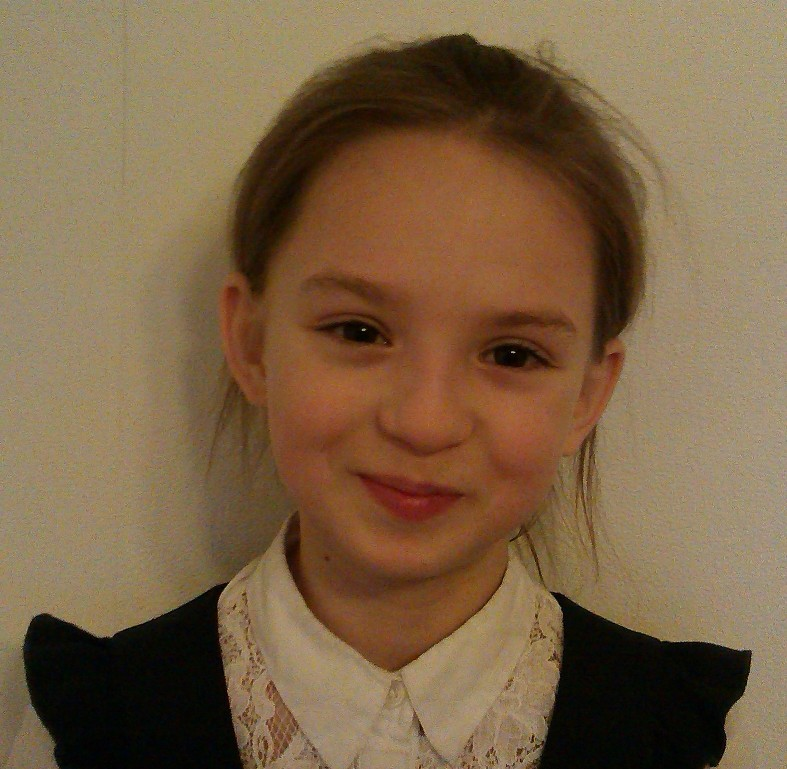
\includegraphics[width=.8\textwidth]{fig/nastyaOfficial}
                    \end{center}
                }
                \only<2>{
                    \begin{center}
                        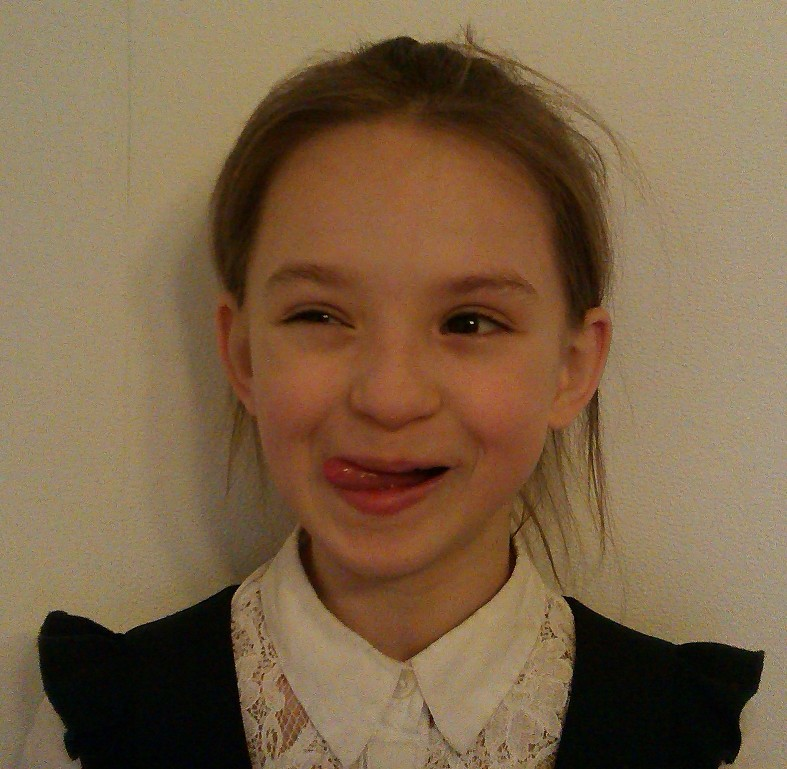
\includegraphics[width=.8\textwidth]{fig/nastyaFox}
                    \end{center}
                }
            }
            \mode<handout> {
                \begin{center}
                    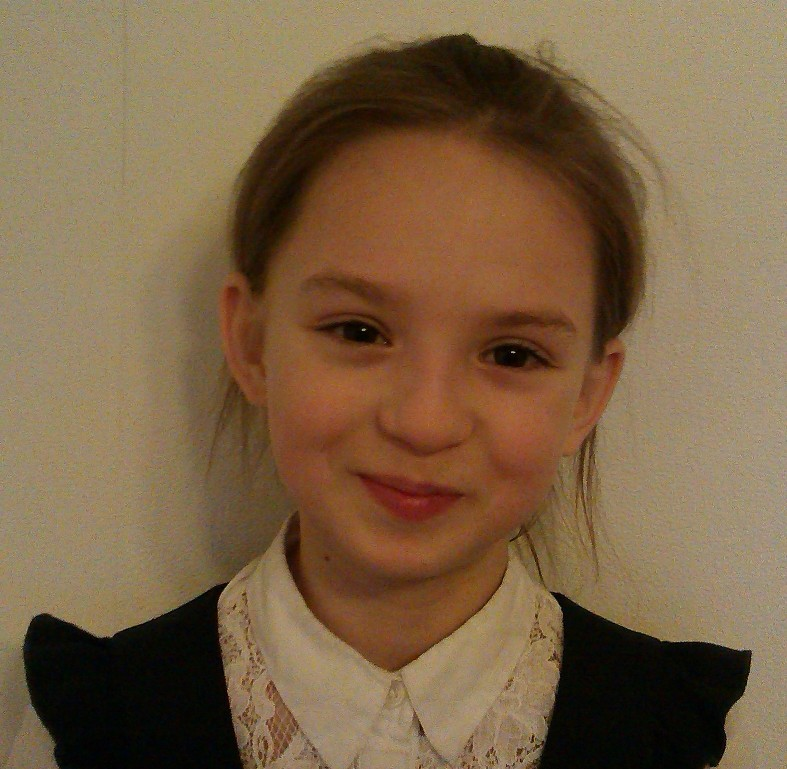
\includegraphics[width=.8\textwidth]{fig/nastyaOfficial}
                \end{center}
            }
        
        \column{.75\textwidth}
            \alert{Автор и докладчик}: Усольцева Настя, дипломированный хулиган, кандидат привниматических наук, почётный член академии нытиков.
    \end{columns}    
    
    \par\bigskip
    
    \alert{Техническая и моральная поддержка}:
    \begin{itemize}
        \item папа Миша;
        \item мама Оля;
        \item сестра Полина;
        \item кошки (2 шт.);
        \item \alert{КОТ};
        \item собака.
    \end{itemize}
\end{frame}

\begin{frame}
    \frametitle{Аннотация}
    
    В работе даётся определение и рассматриваются виды \alert{привниматических устройств} (далее просто: \alert{устройства}).
    
    \par\bigskip
    
    Приводятся \alert{особенности и правила} использования таких устройств. 
    
    \par\bigskip

    Анализируются уже \alert{существующие образцы} устройств.

    \par\bigskip
    
    Разрабатывается и испытывается <<вниматомёт>> \alert{\myDevice} и даётся прогноз направлений развития привниматических устройств\footnote{Исходные тексты презентации и программ доступны в сети Интернет по адресу \url{https://github.com/mmshihov/informatics/tree/master/lections/presentation/F0-app-attention}}.
\end{frame}

\begin{frame}
    \frametitle{Введение и обоснование актуальности}
    
    \alert{Внимание} --- это желанный духовный ресурс, которого на всех не хватает. 

    \par\bigskip
    Невнимательных и нечутких людей становится всё больше. Виной тому множество причин. Но основная --- столь ценное внимание всё чаще рассеивается на \alert{неживые} объекты, такие как телевизоры, мобильные телефоны и компьютеры.

    \par\bigskip

    Поэтому внимание современного человека приходится прямо-таки \alert{завоёвывать}!

    \par\bigskip

    Привниматические устройства --- помощники в этой войне. И их разработка --- это актуальная проблема нашего времени.
\end{frame}

\begin{frame}
    \frametitle{Определение}
    
    \begin{block}{}
        \par\bigskip
        \alert{$\overbrace{\text{ПРИ}}\overbrace{\text{ВНИ}}\overbrace{\text{МАТИЧЕСКОЕ}}$} устройство --- это устройство, 
        \begin{itemize}
            \item \alert{ПРИ}влекающее 
            \item \alert{ВНИ}мание 
            \item авто\alert{МАТИЧЕСКИ}.
        \end{itemize}
    \end{block}
\end{frame}
    
    
\begin{frame}
    \frametitle{Цель и задачи}
    
    \begin{block}{Цель:}
        \begin{center}
            найти \alert{лучшее} привниматическое устройство.
        \end{center}
    \end{block}
    
    \par\bigskip
    
    \begin{block}{Задачи:}
        \begin{itemize}
            \item исследовать существующие образцы привниматических устройств; 
            \item cоздать и испытать собственный образец;
            \item обобщить результаты проведенных испытаний.
        \end{itemize}
    \end{block}
\end{frame}


\section{Исследование существующих образцов}

\subsection{Характеристики привниматических устройств}

\begin{frame}
    \frametitle{Характеристики привниматических устройств}
    
    Привниматическое устройство должно.
    \begin{itemize}
        \item Быть безопасным для здоровья человека. Для краткости назовем характеристику: \alert{Безвредно}.
        
        \item Максимально раздражать. \alert{Эффектно}.  
        
        \item Давать возможность скрытного использования. \alert{Скрытно}.  
        
        \item Не затруднять движений. \alert{Носимо}.
        
        \item Иметь низкую стоимость эксплуатации. \alert{Дёшево}. 
        
        \item Быть простым в использовании. \alert{Просто}.

        \item Быть уникальным в своем роде. \alert{Редко}.
    \end{itemize}
\end{frame}

\begin{itemize}
    \item \alert{Безвредно}. Ведь нужно внимание, а не труп. Труп обычно совершенно невнимателен.
    
    \item \alert{Эффектно}. Обида --- это тоже внимание. На войне как на войне.
    
    \item \alert{Скрытно}. Или хотя бы возможность сказать "Ой, я случайно...".
    
    \item \alert{Носимо}. Потому что иногда от внимания некоторых приходится спасаться бегством.
    
    \item \alert{Дёшево}. Тратить на патроны больше средств, чем получишь внимания --- бессмысленно.
    
    \item \alert{Просто}. Иначе придется не купаться во внимании других, а уделять все свое внимание оружию.

    \item \alert{Редко}. Иначе соперник тут же использует свое такое же оружие и перетянет внимание на себя.
\end{itemize}


\subsection{Оценка характеристик}

\begin{frame}
    \frametitle{Оценка характеристик}

    \begin{columns}
        \column{.45\textwidth}
            Оценить каждую характеристику можно по пятибалльной шкале и свести в таблицу. Например, оценка привлекающего устройства \alert{"букет цветов"} приводится в правой части слайда. Общую оценку можно вычислить по формуле \eqref{eq:average}.
            \begin{equation}
                \label{eq:average}
                \text{Итого}={\displaystyle\sum_{i=1}^{7}\text{Оценка}_i}
            \end{equation}
            
            
        \column{.50\textwidth}
            \begin{center}
                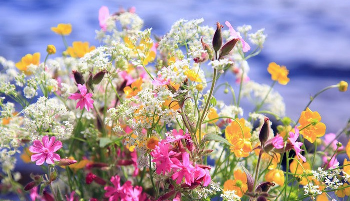
\includegraphics[width=.4\textheight]{fig/flowers}
                
                \begin{tabular}{c|c}
                    \hline\hline
                    Характеристика              & Оценка\\ \hline\hline
                    Безвредно                   & 4 \\
                    Эффектно                    & 1 \\
                    Скрытно                     & 2 \\
                    Носимо                      & 3 \\
                    Дёшево                      & 3 \\
                    Просто                      & 3 \\ 
                    Редко                       & 1 \\ \hline
                    \multicolumn{1}{r|}{Итого:} & $17$ \\
                \end{tabular}
            \end{center}
    \end{columns}    
\end{frame}

Чтобы сделать обоснованные выводы ученому приходится опираться на математику и логику. Чтобы обоснованно выбрать лушее оружие, нам нужно сравнить характеристики разных видов оружия. 

Характеристик много, а значит нужно придумать как свести такой набор оценок к одному числу. Мы решили просто сложить все семь оценок и получить суммарное количество баллов. Для букета цветов, как видно, получилось 18.
\par\bigskip

\subsection{Оценка существующих моделей}

\begin{frame}  %айфоня
    \begin{columns}
        \column{.50\textwidth}
            \begin{center}
                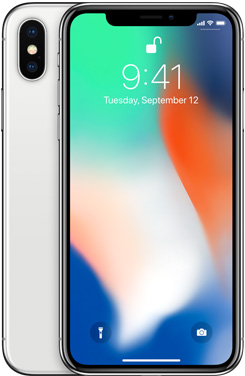
\includegraphics[height=.8\textheight]{fig/iphoneX}
            \end{center}
            
        \column{.40\textwidth}
            \begin{center}
                \begin{tabular}{c|c}
                    \hline\hline
                    Характеристика              & Оценка\\ \hline\hline
                    Безвредно                   & 1 \\
                    Эффектно                    & 1 \\
                    Скрытно                     & 1 \\
                    Носимо                      & 5 \\
                    Дёшево                      & 0 \\
                    Просто                      & 2 \\ 
                    Редко                       & 1 \\ \hline
                    \multicolumn{1}{r|}{Итого:} & $11$ \\
                \end{tabular}
            \end{center}
    \end{columns}    
    
    Отвлекает \alert{всё} внимание от \alert{вас} на себя! Это \alert{не помощник} (см. оценки), а \alert{соперник}!
\end{frame}

%Смартфон - это маленький компьютер, созданный для помощи деловым людям. Он используется для организации работ, планирования времени, доступа к Интернет, мобильной связи, и т.д. И, конечно, для игр, которые, безусловно, нужны для отдыха.

%Человек, использующий смартфон в основном для игр, обычно и не подозревает о его реальных возможностях. Индустрия же компьютерных игр огромна и создает просто потрясающие игры.

%Игра --- это сказочный мир (теперь помещающийся в ладони), который не требует к себе ответственного отношения, в отличие от реального мира. Именно этим она успешно \alert{отвлекает} внимание игрока от реальной жизни, а порой и вовсе стирает грань между иллюзией и реальностью в неокрепших умах.

%Смартфон-игрушка скорее отвлекает внимание на себя, а не привлекает его к хозяину. Он обычно намного интереснее своего хозяина. Компьютерные игры --- это современные соперники в борьбе за внимание человека.

Айфон получает 11 баллов.

\begin{frame}  %духовая трубочка
    \begin{columns}
        \column{.50\textwidth}
            \begin{center}
                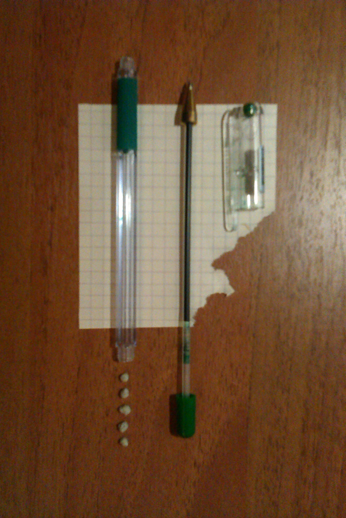
\includegraphics[width=.8\textwidth]{fig/airpipe}
            \end{center}
            
        \column{.40\textwidth}
            \begin{center}
                \begin{tabular}{c|c}
                    \hline\hline
                    Характеристика              & Оценка\\ \hline\hline
                    Безвредно                   & 4 \\
                    Эффектно                    & 5 \\
                    Скрытно                     & 5 \\
                    Носимо                      & 5 \\
                    Дёшево                      & 5 \\
                    Просто                      & 4 \\ 
                    Редко                       & 0 \\ \hline
                    \multicolumn{1}{r|}{Итого:} & $28$ \\
                \end{tabular}
            \end{center}
    \end{columns}    
\end{frame}

Духовая трубочка (кому объяснить как пользоваться?) получает 28 баллов.

\begin{frame} % рогатка из резиночки
    \begin{columns}
        \column{.50\textwidth}
            \begin{center}
                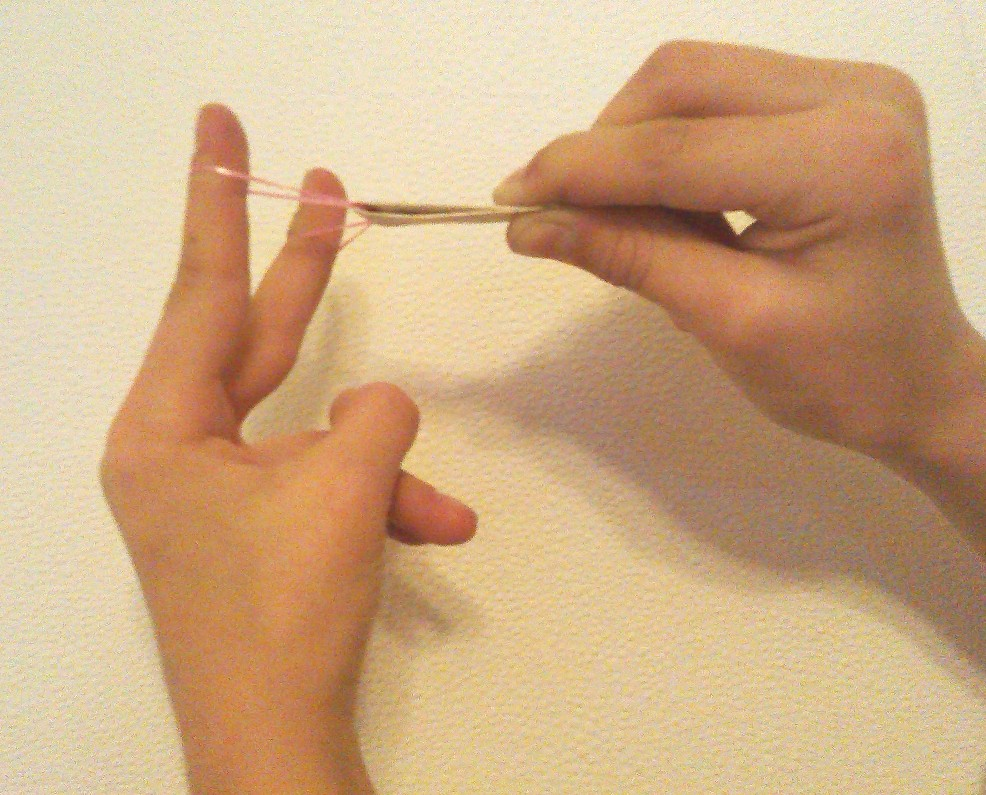
\includegraphics[width=\textwidth]{fig/slingshot}
            \end{center}
            
        \column{.40\textwidth}
            \begin{center}
                \begin{tabular}{c|c}
                    \hline\hline
                    Характеристика              & Оценка\\ \hline\hline
                    Безвредно                   & 4 \\
                    Эффектно                    & 5 \\
                    Скрытно                     & 3 \\
                    Носимо                      & 3 \\
                    Дёшево                      & 5 \\
                    Просто                      & 4 \\ 
                    Редко                       & 0 \\ \hline
                    \multicolumn{1}{r|}{Итого:} & $24$ \\
                \end{tabular}
            \end{center}
    \end{columns}    
\end{frame}

Рогатка из резиночки получает 24 балла.

\begin{frame} % резиночки сами по себе
    \begin{columns}
        \column{.50\textwidth}
            \begin{center}
                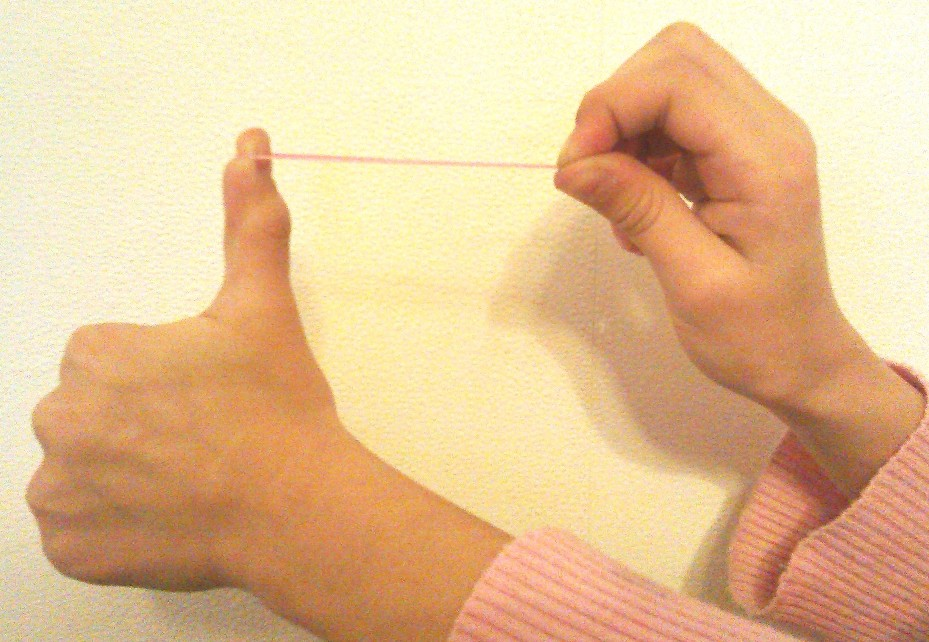
\includegraphics[width=\textwidth]{fig/elastic}
            \end{center}
            
        \column{.40\textwidth}
            \begin{center}
                \begin{tabular}{c|c}
                    \hline\hline
                    Характеристика              & Оценка\\ \hline\hline
                    Безвредно                   & 4 \\
                    Эффектно                    & 5 \\
                    Скрытно                     & 5 \\
                    Носимо                      & 5 \\
                    Дёшево                      & 4 \\
                    Просто                      & 4 \\ 
                    Редко                       & 0 \\ \hline
                    \multicolumn{1}{r|}{Итого:} & $27$ \\
                \end{tabular}
            \end{center}
    \end{columns}    
\end{frame}

Стрельба резиночками для плетения (в прошлом году стала бедствием нашей школы) получает 27 баллов.

\begin{frame}
    \begin{center}
        Видно, что существующие образцы можно улучшить. 
        
        \par\bigskip
        
        Разработаем свой образец.
        
        \par\bigskip

        За основу возмьмем стрельбу резиночками и улучшим их невысокие характеристики \alert{Просто} и \alert{Редко}.
    \end{center}
\end{frame}

По результатам наших исследований стрельба резиночками является наиболее совершенным из рассмотренных видов оружия. Она получила максимальные 27 баллов. Совершенству нет предела и мы попробуем создать собственный образец оружия.
\par\bigskip

\section{Создание и испытание нового образца}

\begin{frame}
    \frametitle{\myDevice}
    
    \begin{center}
        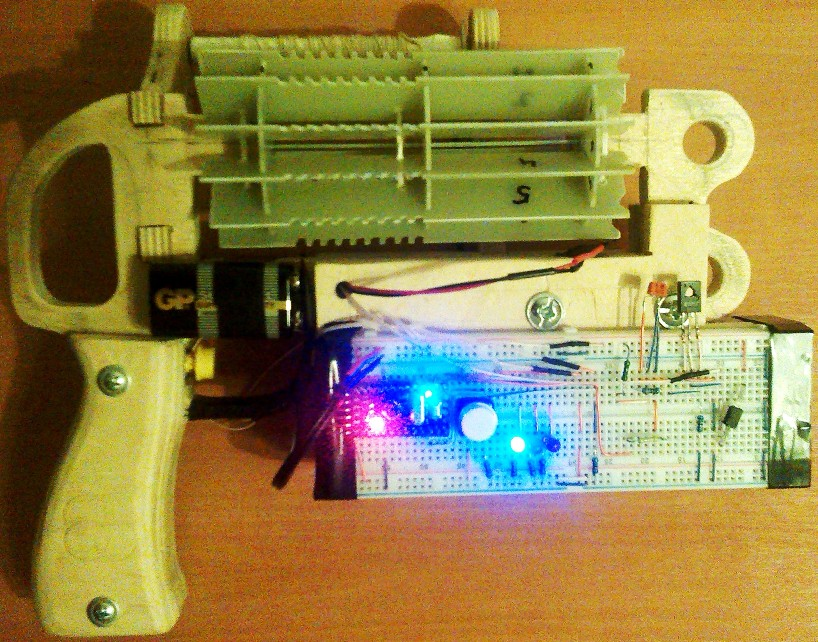
\includegraphics[width=0.7\textwidth]{fig/device}
    \end{center}
\end{frame}

На слайде представлен внешний вид созданного вниматомета {\myDevice}. Он позволяет вести автоматическую стрельбу резиночками в разных режимах.

\begin{frame}
    \frametitle{Режимы работы \myDevice}
    \framesubtitle{Переключаются отдельной кнопкой}
    
    \begin{itemize}
        \item Вялый:
            \begin{center}
                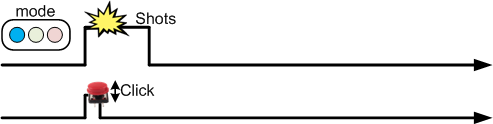
\includegraphics[width=0.5\textwidth]{fig/modeSlow}
            \end{center}
            
        \item Импульсный:
            \begin{center}
                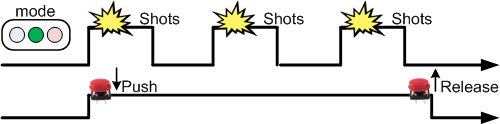
\includegraphics[width=0.5\textwidth]{fig/modePulse}
            \end{center}
            
        \item Шквал:
            \begin{center}
                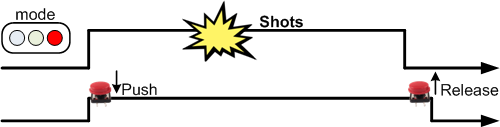
\includegraphics[width=0.5\textwidth]{fig/modeStorm}
            \end{center}
    \end{itemize}    
\end{frame}

Режими работы последовательно переключаются отдельной кнопкой (показываем на самом пистолете). 

\begin{itemize}
    \item Вялый (горит синий светодиод) - на одно нажатие курка следует серия выстрелов.
    \item Импульсный (горит зеленый светодиод) - пока удерживается курок, {\myDevice} повторяются серия выстрелов - пауза и т.д.
    \item Шквал (горит красный светодиод) - пока удерживается курок, {\myDevice} стреляет непрерывно.
\end{itemize}    


\subsection{Устройство}

\begin{frame}
    \frametitle{Механика \myDevice}
    
    \begin{center}
        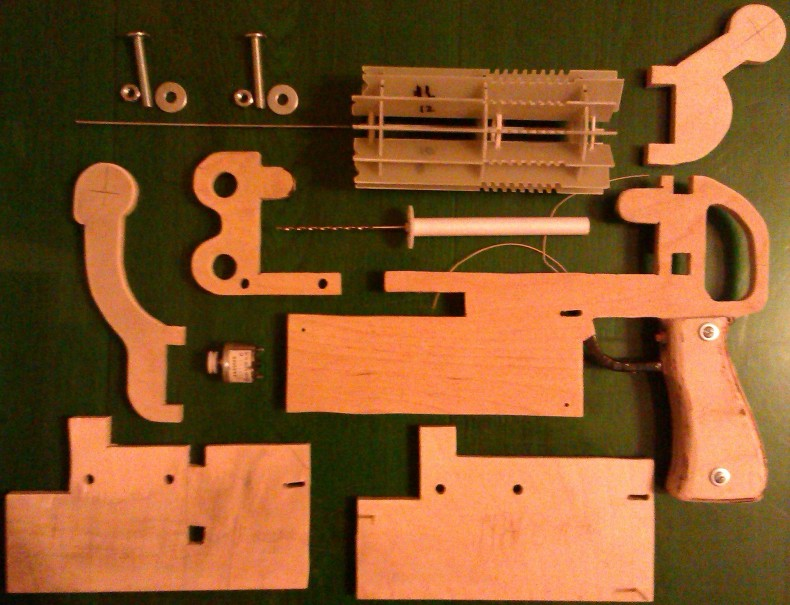
\includegraphics[width=0.7\textwidth]{fig/mechanics}
    \end{center}
\end{frame}

На слайде показана механическая часть {\myDevice}. Электромоторчик приводит в действие спусковой механизм. А моторчиком управляет электроника.

\begin{frame}
    \frametitle{Электроника {\myDevice} --- схема}
    
    \begin{center}
        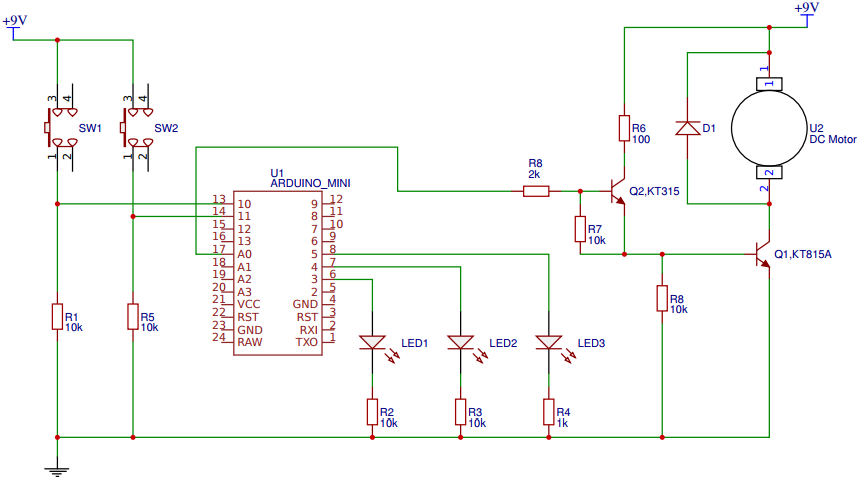
\includegraphics[width=0.99\textwidth]{fig/eScheme}
    \end{center}
\end{frame}

Вначале инженер рисует электронную схему, которая условно изображает как соединить проводами разные электронные элементы, такие как (показываем на слайде): моторчики, кнопки, светодиоды, сопротивления, транзисторы. Самый сложный элемент нашей схемы --- микрокомпьютер, упрвляющий работой вниматомета.

\begin{frame}
    \frametitle{Электроника {\myDevice} --- макет}
    
    \begin{center}
        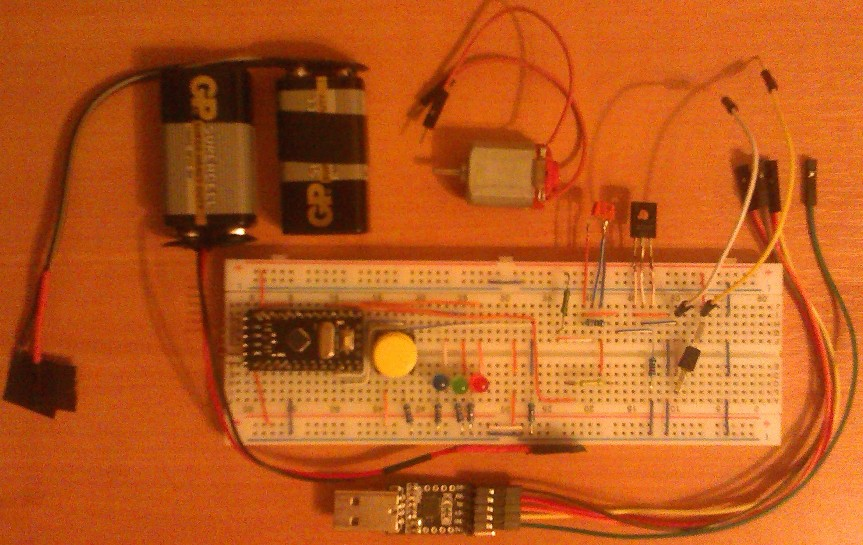
\includegraphics[width=0.8\textwidth]{fig/eModel}
    \end{center}
\end{frame}

Первый, опытный, образец обычно собирают быстро и грубо. Для этого используют макетные платы, которые позволяют собирать электронные схемы очень быстро. Поэтому {\myDevice} выглядит ужасно. На слайде можно можно увидеть уже собранную схему, которая была на предыдущем слайде. Вот как выглядят (прим: показываем на картинке) моторчик, кнопки, микрокомпьютер, транзисторы, сопротивления, светодиоды на самом деле.

\begin{frame}
    \frametitle{Программирование контроллера \myDevice}
    
    \begin{center}
        
\includegraphics[width=0.4\textwidth]{fig/programming}
    \end{center}
\end{frame}

Режимами работы и стрельбой управляет программа, загруженная в микрокомпьютер.

Эта программа была создана на обычном компьютере и с помощью специального устройства - программатора - перемещена в микрокомпьютер. 

На слайде показан специальный редактор, в котором программист пишет такие программы.

Когда микрокомпьютер начинает выполнять программу, вниматомет "оживает".

\begin{frame}
    \frametitle{Смета проекта \myDevice}
    
    \begin{center}
        \begin{tabular}{l|c|c|l}
            \hline\hline
            Деталь & Кол-во,шт. & Цена,руб. & Примечание \\
            \hline\hline
            Контроллер & 1  & 70   & Arduino Pro Mini,5V,16MHz\\
            Светодиод  & 3  & 0.50 & Красный, синий, зелёный\\
            Breadboard & 1  & 50   & Чтобы не паять детали\\
            Моторчик   & 1  & 50   & 4-9V, max 1A, 800 RPM\\
            Шестерёнки & 2  & 5    & Крутить обойму\\
            Батарейка  & 2  & 40   & Крона, 9V, питание схемы\\
            Провод     & -  & 0    & Соединять элементы\\
            Транзистор & 2  & 0    & Управлять моторчиком\\
            Фанера     & -  & 0    & Для корпуса\\
            Текстолит  & -  & 0    & Для ствола\\
            Резиночки  & 84 & 0    & Патроны\\ \hline
            \multicolumn{2}{r|}{Итого(\alert{без учёта работ}):} & \multicolumn{1}{c}{\alert{$261.50$}} & \\
        \end{tabular}
    \end{center}
\end{frame}

Смета отражает стоимость создания вниматомета без учета оплаты труда разработчиков - только материалы и детали.


\subsection{Испытания \myDevice}

\begin{frame}
    \frametitle{Испытания \myDevice}
    \begin{center}
        В ходе испытаний ни одно живое существо не пострадало.

        Физически\ldots    
    \end{center}    
\end{frame}

\begin{frame}
    \frametitle{Испытание на котах}
    
    \begin{center}
        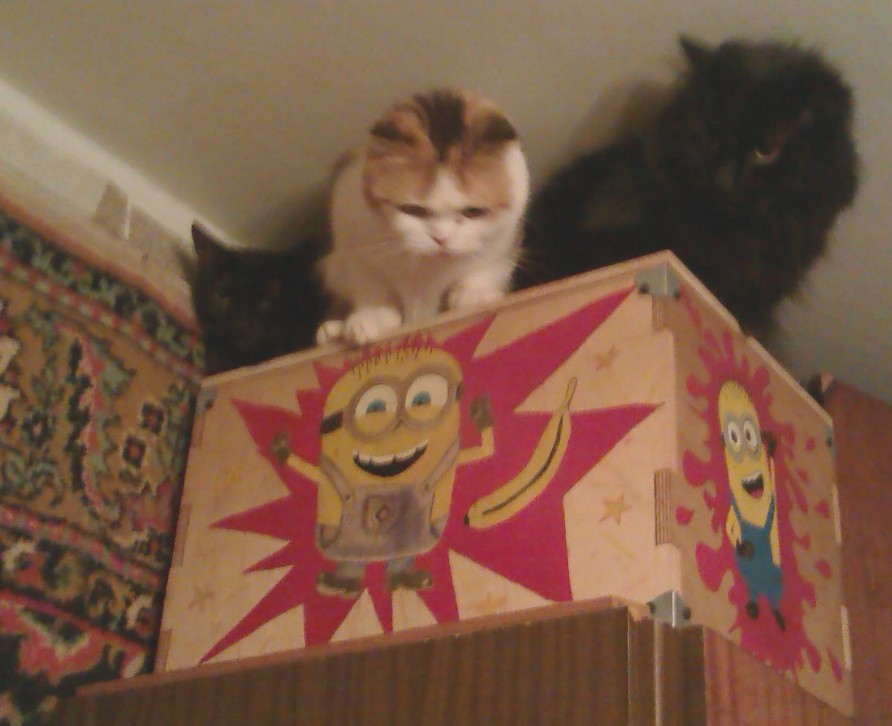
\includegraphics[width=0.7\textwidth]{fig/cats}
    \end{center}
\end{frame}

\begin{frame}
    \frametitle{Испытание на собаке}
    
    \begin{center}
        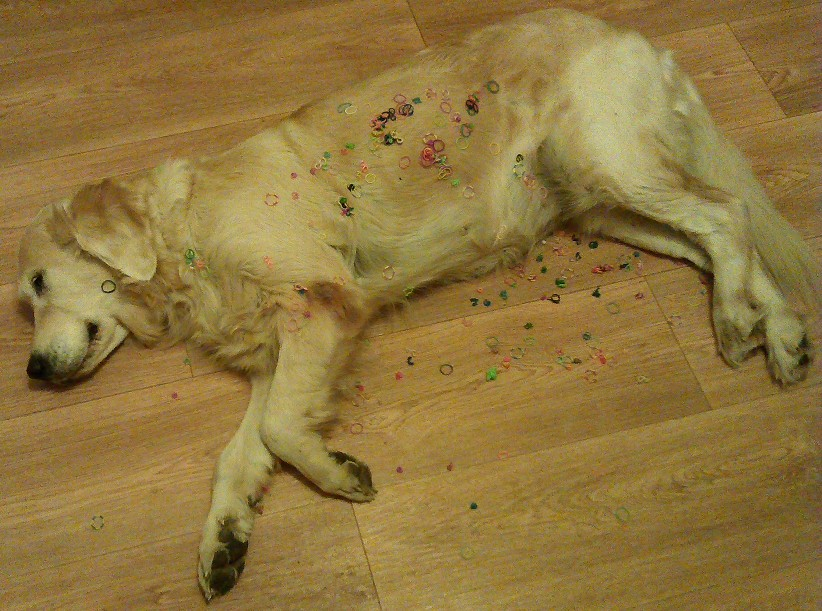
\includegraphics[width=0.75\textwidth]{fig/dog}
    \end{center}
\end{frame}

\begin{frame}
    \frametitle{Испытание на сестре}
    \framesubtitle{Без паники! Сестра помогала <<отфотошопить>> мою фотографию. Спасибо ей!}
    
    \begin{center}
        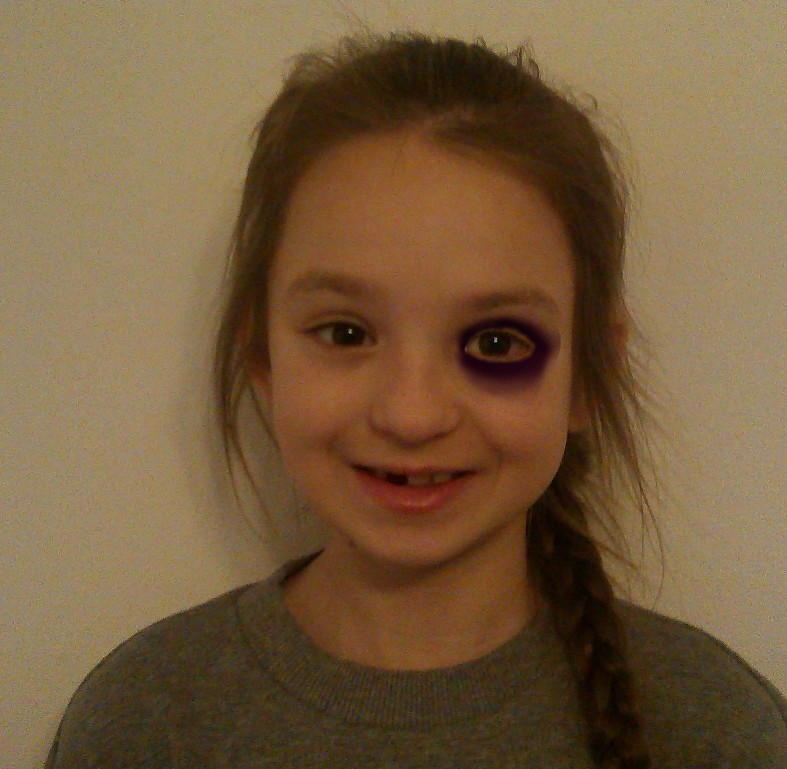
\includegraphics[width=0.55\textwidth]{fig/nastyaWork}
    \end{center}
\end{frame}

\begin{frame}
    \frametitle{Испытание на родителях}
    
    \begin{center}
        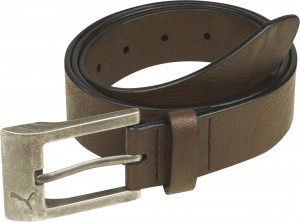
\includegraphics[width=.6\textwidth]{fig/belt}
    \end{center}
    
    Испытание на родителях решено не проводить\ldots
\end{frame}


\section{Оценки и выводы}

\begin{frame}
    \frametitle{Сравнительная оценка характеристик \myDevice}
    
    \begin{columns}
        \column{.30\textwidth}
            \begin{center}
                \scalebox{.15}{\rotatebox{90}{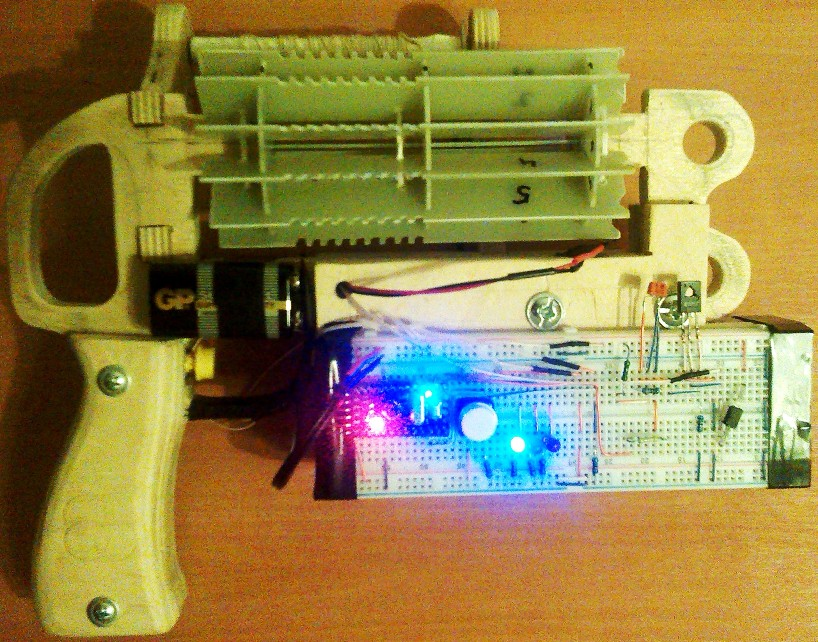
\includegraphics{fig/device}}}
            \end{center}
            
        \column{.70\textwidth}
            \begin{center}
                \begin{tabular}{c|c|c}
                    \hline\hline
                    Характеристика              & {\myDevice}   & Резиночки\\ \hline\hline
                    Безвредно                   & 4             & 4\\
                    Эффектно                    & 5             & 5\\
                    Скрытно                     & \alert{3}     & 5\\
                    Носимо                      & \alert{3}     & 5\\
                    Дёшево                      & \alert{3}     & 4\\
                    Просто                      & 5             & \alert{4}\\ 
                    Редко                       & 5             & \alert{0}\\ \hline
                    \multicolumn{1}{r|}{Итого:} & $28$          & $27$ \\
                \end{tabular}
            \end{center}
    \end{columns}
\end{frame}

Оценка созданного оружия на практике оказалась невысокой. Мы улучшили характеристики \alert{Просто} (стрельба сводится к нажатию кнопки) и \alert{Редко} (на руках единственный в мире {\myDevice}). Однако это привело к ухудщению других характеристик: Скрытно, Носимо и Дёшево.

Ценность практического результата оказалась невелика, но проведенные исследования позволяют сделать однозначные научные выводы!


\subsection{Вывод по использованию устройства}

\begin{frame}
    \frametitle{Главный вывод}
    
    \begin{block}{Главный вывод}
        Привниматическое устройство \alert{не должно} быть направлено на того, чьё внимание нужно привлечь. 
    \end{block}
    
    \par\bigskip
    
    Лучше использовать его вместе, в дружеской игре --- тогда внимание будет \alert{взаимным} и \alert{добрым}.
\end{frame}


\subsection{Самое мощное\ldots}

\begin{frame}
    \frametitle{Заключение}
    
    Обобщив полученный опыт, можно с уверенностью утверждать, что:
    
    \begin{block}{}
        Самое мощное и \alert{единственное настоящее} привниматическое устройство --- это умный, сильный, увлекающийся, любопытный, а главное --- \alert{внимательный} к окружающему миру \alert{ЧЕЛОВЕК}!
    \end{block}
    
    {\myDevice} оказался неудачным экспериментом, но сама работа над ним позволила вырасти над собой и понять, что

    \begin{block}{}
        никакие внешние устройства для привлекательности \alert{НЕ НУЖНЫ}; задача привлечения внимания решается 
        \begin{center}
            \alert{усовершенствованием самого себя}!
        \end{center}
    \end{block}
\end{frame}

    
\subsection{Новая цель}

\begin{frame}
    \frametitle{Новая цель и направления развития}
    
    \begin{block}{Новая цель}
        \begin{center}
            \alert{Саморазвитие}!!!
        \end{center}
    \end{block}
    
    Стать \alert{привлекательным} можно, развиваясь в следующих направлениях:
    \begin{itemize}
        \item в искусстве (музыки, танца, рисования, лепки, рукоделия,\ldots);
        \item в науке (физике, математике, химии, биологии, психологии,\ldots);
        \item в спорте (гимнастике, атлетике, плавании, боевых искусствах,\ldots);
        \item в помощи (людям, животным, растениям, чистоте улиц,\ldots);
        \item в медиа (прозе, стихах, журналистике, блогинге,\ldots);
        \item и т.д.
    \end{itemize}
    
    \begin{block}{}
        \begin{center}
            \alert{Один} человек может развиваться во \alert{многих} направлениях!
        \end{center}
    \end{block}
    
\end{frame}


\appendix

\begin{frame}
    \frametitle{Список использованной литературы}

    Уверены, пригодится \alert{всем}:
    \begin{itemize}
        \item создание характера в \cite{bib:kovey:sevenHabits};
        \item живой Русский язык в \cite{bib:gal:WordLiveAndDeath}.
    \end{itemize}
    
    \par\bigskip
    
    Только тем, кому интересно, что такое:
    \begin{itemize}
        \item основы программирования \cite{bib:kernigan:practice};
        \item микроконтроллеры и электроника \cite{bib:petin:Arduino}.
    \end{itemize}
\end{frame}

\begin{frame}{Список литературы}
    \bibliographystyle{unsrt}
    \bibliography{./../../../bibliobase}
\end{frame}

\begin{frame}
    \begin{center}
        \resizebox{\textwidth}{!}{Благодарю за \alert{внимание}!}
    \end{center}
    
    \par\bigskip
    
    \begin{center}
        Вопросы?
    \end{center}
    
\end{frame}

\end{document}